%! Suppress = MissingImport
%! Suppress = TooLargeSection
%! Suppress = SentenceEndWithCapital
%! Suppress = LineBreak
%! Suppress = MissingLabel
%! Suppress = Unicode

\documentclass[main.tex]{subfiles}

\begin{document}

    \section{Relacyjny model danych, normalizacja relacji (w szczególności algorytm doprowadzenia relacji do postaci Boyce’a-Codda), przykłady.}
    \section{Indeksowanie w bazach danych: drzewa B+, tablice o organizacji indeksowej, indeksy haszowe, mapy binarne.}
    \section{Podstawowe cechy transakcji (ACID). Metody sterowania współbieżnością transakcji, poziomy izolacji transakcji, przykłady.}
    \section{Złączenia, grupowanie, podzapytania w języku SQL.}

    \newpage

    \section{Szeregowalność harmonogramów w bazach danych.}

    Dla uproszczenia rozważań przyjmiemy, że operacja zapisu powoduje natychmiastowy zapis elementu danych na dysk.\\

    \textbf{Przykład}:\\

    $T_1$ : transfer 50 zł z konta A na konto B

    $T_2$ : transfer 10\% z A na konto B

    Przed rozpoczęciem transakcji: A = 1000 zł, B = 2000 zł

    Wymaganie spójności: $( A + B )_{\text{przed transakcją}} = ( A + B )_{\text{po transakcji}}$

    \begin{table}[H]
        \begin{center}
            \begin{tabular}{p{8cm} p{8cm}}
                $T_1$ & $T_2$ \\
                read (A) & read (A)\\
                A := A - 50 & temp := A * 0.1\\
                write (A) & A := A - temp\\
                read (B) & write (A)\\
                B := B + 50 & read (B)\\
                write (B) & B := B + temp\\
            \end{tabular}
        \end{center}
    \end{table}

    \newpage

    \noindent \textbf{Harmonogram S1 - szeregowy}, $<T_1, T_2>$ (czyt: najpierw operacje z $T_1$, potem operacje z $T_2$).
    \begin{table}[H]
        \begin{center}
            \begin{tabular}{| p{6cm} | p{6cm} |}
                \hline
                $T_1$ & $T_2$\\
                \hline
                \hline
                read (A) &\\
                \hline
                A := A - 50 &\\
                \hline
                write (A) &\\
                \hline
                read (B) &\\
                \hline
                B := B + 50 &\\
                \hline
                write (B) &\\
                \hline
                & read (A)\\
                \hline
                & temp := A * 0.1\\
                \hline
                & A := A - temp\\
                \hline
                & write (A)\\
                \hline
                & read (B)\\
                \hline
                & B := B + temp\\
                \hline
                & write (B)\\
                \hline
            \end{tabular}
        \end{center}
    \end{table}

    Po transakcji: A = 855, B = 2145

    Wymaganie spójności:
    $( A + B )_{\text{przed transakcją}} = ( A + B )_{\text{po transakcji}} = 3000$\\

    \newpage

    \noindent \textbf{Harmonogram S2 - współbieżny}, równoważny w sensie wyniku harmonogramowi S1.
    \begin{table}[H]
        \begin{center}
            \begin{tabular}{| p{6cm} | p{6cm} |}
                \hline
                $T_1$ & $T_2$\\
                \hline
                \hline
                read (A) &\\
                \hline
                A := A - 50 &\\
                \hline
                write (A) &\\
                \hline
                & read (A)\\
                \hline
                & temp := A * 0.1\\
                \hline
                & A := A - temp\\
                \hline
                & write (A)\\
                \hline
                read (B) &\\
                \hline
                B := B + 50 &\\
                \hline
                write (B) &\\
                \hline
                & read (B)\\
                \hline
                & B := B + temp\\
                \hline
                & write (B)\\
                \hline
            \end{tabular}
        \end{center}
    \end{table}

    Po transakcji: A = 855, B = 2145. Zachowany warunek spójności.\\

    \noindent \textbf{Harmonogram S3 - współbieżny}.
    \begin{table}[H]
        \begin{center}
            \begin{tabular}{| p{6cm} | p{6cm} |}
                \hline
                $T_1$ & $T_2$\\
                \hline
                \hline
                read (A) &\\
                \hline
                A := A - 50 &\\
                \hline
                & read (A)\\
                \hline
                & temp := A * 0.1\\
                \hline
                & A := A - temp\\
                \hline
                & write (A)\\
                \hline
                & read (B)\\
                \hline
                write (A) &\\
                \hline
                read (B) &\\
                \hline
                B := B + 50 &\\
                \hline
                write (B) &\\
                \hline
                & B := B + temp\\
                \hline
                & write (B)\\
                \hline
            \end{tabular}
        \end{center}
    \end{table}

    Po transakcji: A = 950, B = 2100.

    \textbf{Niespójny stan bazy danych!} - $( A + B )_{\text{przed transakcją}} = 300 ~ != ~ ( A + B )_{\text{po transakcji}} = 3050$\\
    $T_1$ nadpisuje wartość A zapisaną przez $T_2$.

    \subsection{Szeregowalność konfliktowa.}
    Uprościmy harmonogramy do operacji odczytu i zapisu.\\

    \noindent Jeszcze raz harmonogram \textbf{S2}:
    \begin{table}[H]
        \begin{center}
            \begin{tabular}{| p{0.8cm} | p{6cm} | p{6cm} |}
                \hline
                & $T_1$ & $T_2$\\
                \hline
                \hline
                1 & read (A) &\\
                \hline
                2 & write (A) &\\
                \hline
                3 & & read (A)\\
                \hline
                4 & & write (A)\\
                \hline
                5 & read (B) &\\
                \hline
                6 & write (B) &\\
                \hline
                7 & & read (B)\\
                \hline
                8 & & write (B)\\
                \hline
            \end{tabular}
        \end{center}
    \end{table}

    Operacje konfliktowe - 2 i 3, 5 i 7 - odnoszą się z różnych transakcji do tej samej zmiennej.\\

    \noindent Weźmy harmonogram \textbf{S4} - powstały z harmonogramu S2 przez zamianę kolejności instrukcji niekonfliktowych.
    \begin{table}[H]
        \begin{center}
            \begin{tabular}{| p{0.8cm} | p{6cm} | p{6cm} |}
                \hline
                & $T_1$ & $T_2$\\
                \hline
                \hline
                1 & read (A) &\\
                \hline
                2 & write (A) &\\
                \hline
                3 & & read (A)\\
                \hline
                4 & \textbf{read (B)} &\\
                \hline
                5 & & \textbf{write (A)}\\
                \hline
                6 & write (B) &\\
                \hline
                7 & & read (B)\\
                \hline
                8 & & write (B)\\
                \hline
            \end{tabular}
        \end{center}
    \end{table}

    S2 i S4 są \textbf{konfliktowo równoważne}.\\


    \noindent Harmonogram \textbf{S1} z podstawowym operacjami:
    \begin{table}[H]
        \begin{center}
            \begin{tabular}{| p{0.8cm} | p{6cm} | p{6cm} |}
                \hline
                & $T_1$ & $T_2$\\
                \hline
                \hline
                1 & read (A) &\\
                \hline
                2 & write (A) &\\
                \hline
                3 & \textbf{read (B)}&\\
                \hline
                4 & \textbf{write (B)}&\\
                \hline
                5 & & \textbf{read (A)}\\
                \hline
                6 & & \textbf{write (A)}\\
                \hline
                7 & & read (B)\\
                \hline
                8 & & write (B)\\
                \hline
            \end{tabular}
        \end{center}
    \end{table}

    Pogrubione operacje to te, których możemy zmienić kolejność (3 i 4 zamienione z 5 i 6) - otrzymalibyśmy wtedy
    harmonogram S2. Zatem S1 i S2 są \textbf{konfliktowo równoważne}. Ponieważ S1 jest szeregowy, to S2 jest
    \textbf{szeregowalny konfliktowo.}\\

    \textbf{Podsumowując:}
    \begin{center}
        S1 i S2 są konfliktowo równoważne.\\
        S1 i S3 nie są konfliktowo równoważne.\\
        S2 i S4 są konfliktowo równoważne.\\
        S1 jest szeregowy.\\
        S2 i S4 są szeregowalne konfliktowo.\\
    \end{center}

    \subsection{Szeregowalność perspektywiczna.}
    Równoważność perspektywiczna:
    \begin{enumerate}[label=(\Alph*)]
        \item Jeśli w S $T_k$ jest transakcją, która w
        harmonogramie czyta Q jako pierwsza, to w S' $T_k$ musi być transakcją, która czyta Q jako pierwsza.
        \item Jeśli w S $T_i$ czyta Q zapisany przez $T_j$, to w S' $T_i$ czyta Q zapisany przez $T_j$.
        \item Jeśli w S  $T_m$ jest ostatnią transakcją, która
        zapisuje Q, to w S' $T_m$ jest ostatnią transakcją, która zapisuje Q.
    \end{enumerate}

    \noindent \textbf{S1}:
    \begin{table}[H]
        \begin{center}
            \begin{tabular}{| p{6cm} | p{6cm} |}
                \hline
                $T_1$ & $T_2$\\
                \hline
                \hline
                read (A) &\\
                \hline
                write (A) &\\
                \hline
                read (B)&\\
                \hline
                write (B)&\\
                \hline
                & read (A)\\
                \hline
                & write (A)\\
                \hline
                & read (B)\\
                \hline
                & write (B)\\
                \hline
            \end{tabular}
        \end{center}
    \end{table}

    \noindent \textbf{S2}:
    \begin{table}[H]
        \begin{center}
            \begin{tabular}{| p{6cm} | p{6cm} |}
                \hline
                $T_1$ & $T_2$\\
                \hline
                \hline
                & read (A)\\
                \hline
                & write (A)\\
                \hline
                & read (B)\\
                \hline
                & write (B)\\
                \hline
                read (A) &\\
                \hline
                write (A) &\\
                \hline
                read (B)&\\
                \hline
                write (B)&\\
                \hline
            \end{tabular}
        \end{center}
    \end{table}

    \noindent \textbf{S3}:
    \begin{table}[H]
        \begin{center}
            \begin{tabular}{| p{6cm} | p{6cm} |}
                \hline
                $T_1$ & $T_2$\\
                \hline
                \hline
                read (A) &\\
                \hline
                write (A) &\\
                \hline
                & read (A)\\
                \hline
                & write (A)\\
                \hline
                read (B)&\\
                \hline
                write (B)&\\
                \hline
                & read (B)\\
                \hline
                & write (B)\\
                \hline
            \end{tabular}
        \end{center}
    \end{table}

    S1: $<T_1, T_2>$ i S2: $<T_2, T_1>$ \textbf{nie są równważnie perspektywicznie}. Nie jest spełniony warunek (B):
    w S1 $T_2$ czyta A zapisane przez $T_1$, ale to samo nie zachodzi w S2.\\

    S1: $<T_1, T_2>$ \textbf{jest równoważny perspektywicznie} S3.\\

    \noindent \textbf{S4}:
    \begin{table}[H]
        \begin{center}
            \begin{tabular}{| p{4cm} | p{4cm} | p{4cm} |}
                \hline
                $T_3$ & $T_4$ & $T_5$\\
                \hline
                \hline
                read(Q) &&\\
                \hline
                & write(Q) &\\
                \hline
                write(Q) &&\\
                \hline
                && write(Q)\\
                \hline
            \end{tabular}
        \end{center}
    \end{table}

    S4 \textbf{jest szeregowalny perspketywicznie}, bo jest perspektywicznie równoważny harmonogramowi szeregowemu
    $<T_3, T_4, T_5>$. S4 \textbf{nie jest szeregowalny konfliktowo}, bo nie możemy pozamieniać kolejności operacji
    - praktycznie wszystkie są konfliktowe.

    \newpage

    \section{Definicja cyfrowego układu kombinacyjnego - przykłady układów kombinacyjnych i ich implementacje.}

    \begin{exercise}
        \textbf{Projektowanie układów kombinacyjnych.} Za pomocą bramek NAND zrealizować układ opisany poniższą tablicą
        prawdy:

        \begin{tabular}{| p{1cm} p{1cm} p{1cm} | p{2cm} |}
            \hline
            \multicolumn{3}{|c|}{Wejścia} & Wyjścia\\
            \hline
            x & y & z & f\\
            \hline
            0 & 0 & 0 & 1\\
            0 & 0 & 1 & 1\\
            0 & 1 & 0 & 1\\
            0 & 1 & 1 & 0\\
            1 & 0 & 0 & 0\\
            1 & 0 & 1 & 0\\
            1 & 1 & 0 & 0\\
            1 & 1 & 1 & 0\\
            \hline
        \end{tabular}
    \end{exercise}

    Na podstawie tablicy prawdy otrzymujemy funkcję logiczną:
    \[f(x,y,z) = \sum (0,1,2) = \bar{x} \bar{y} \bar{z} + \bar{x} \bar{y} z + \bar{x} y \bar{z} = \bar{x} \bar{y} + \bar{x} \bar{z}\]

    Korzystając z praw de Morgana:
    \[f(x,y,z) = \bar{x} \bar{y} + \bar{x} + \bar{z} = \overline{\overline{\bar{x} \bar{y} + \bar{x} + \bar{z}}} = \overline{\overline{\bar{x} \bar{y}} \cdot \overline{\bar{x} \bar{z}}} \]

    Zatem schemat logiczny:

    \begin{figure}[H]
        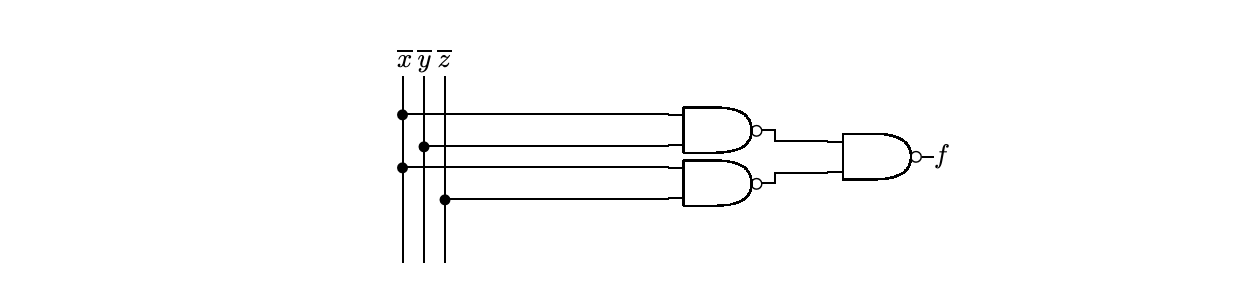
\includegraphics[width=\linewidth]{uk_ex.png}
    \end{figure}

    \newpage

    \section{Definicja cyfrowego układu sekwencyjnego - przykłady układów sekwencyjnych i ich implementacje.}

    \newpage

    \section{Minimalizacja funkcji logicznych.}
    \subsection{Minimalizacja z wykorzystaniem algebry Boole’a}
    \begin{exercise}
        Zminimalizuj funkcję logiczną zadaną poniższą tabelką:
        \begin{table}[H]
            \centering
            \begin{tabular}{|c|c|c|c|}
                \hline
                \textbf{a} & \textbf{b} & \textbf{c} & \textbf{f ( a,b,c )} \\ \hline
                0 & 0 & 0 & 0                    \\ \hline
                0 & 0 & 1 & 0                    \\ \hline
                0 & 1 & 0 & 1                    \\ \hline
                0 & 1 & 1 & 1                    \\ \hline
                1 & 0 & 0 & 1                    \\ \hline
                1 & 0 & 1 & 1                    \\ \hline
                1 & 1 & 0 & 0                    \\ \hline
                1 & 1 & 1 & 0                    \\ \hline
            \end{tabular}
        \end{table}
    \end{exercise}

    \noindent Zapisujemy funkcję w postaci sumy iloczynów poszczególnych argumentów, dla których funkcja przyjmuje wartość 1.
    Oczywiście aby wszystko było zgodne z prawdą, tam gdzie dany argument jest równy 0, musimy go zanegować: \\

    \noindent $\mathbf{f(a, b, c) = (\neg a \wedge b \wedge \neg c) \vee (\neg a \wedge b \wedge c) \vee (a \wedge \neg b \wedge \neg c) \vee (a \wedge \neg b \wedge c)}$ \\

    \noindent Następnie wykorzystując rozdzielność możemy uprościć to wyrażenie: \\

    \noindent $\mathbf{f(a, b, c) = \neg a \wedge (b \wedge \neg c \vee b \wedge c) \vee a \wedge ( \neg b \wedge \neg c \vee \neg b \wedge c) =}$ \\
    \noindent $\mathbf{= \neg a \wedge (b \wedge ( \neg c \vee c)) \vee a \wedge ( \neg b \wedge ( \neg c \vee c))}$ \\

    \noindent Wykorzystując: \\

    \noindent $\mathbf{\neg c \vee c = 1}$ \\
    \noindent $\mathbf{b \wedge 1 = b}$ \\
    \noindent $\mathbf{\neg b \wedge 1 = \neg b}$ \\

    \noindent Otrzymujemy: \\

    \noindent $\mathbf{f(a, b, c) = \neg a \wedge (b \wedge 1) \vee a \wedge ( \neg b \wedge 1) = (\neg a \wedge b) \vee (a \wedge \neg b)}$

    \newpage

    \subsection{Minimalizacja z wykorzystaniem tablic Karnaugha}
    \begin{exercise}
        Uprość funkcję f(x, y, z) = $\sum$(0, 2, 4, 6, 7)
    \end{exercise}

    \noindent W przypadku takiego zapisu funkcji, liczby traktujemy jako zapisane dziesiętnie liczby binarne, w których każdy bit odpowiada danej zmiennej w funkcji
    (najstarszy bit odpowiada pierwszej zmiennej funkcji, itd.) \\
    \noindent Więc dla przykładu 6 odpowiada 110 = $xy\bar{z}$ \\

    \noindent Uzupełniamy tablice Karnaugha dla funkcji 3 zmiennych: \\

    \begin{center}
        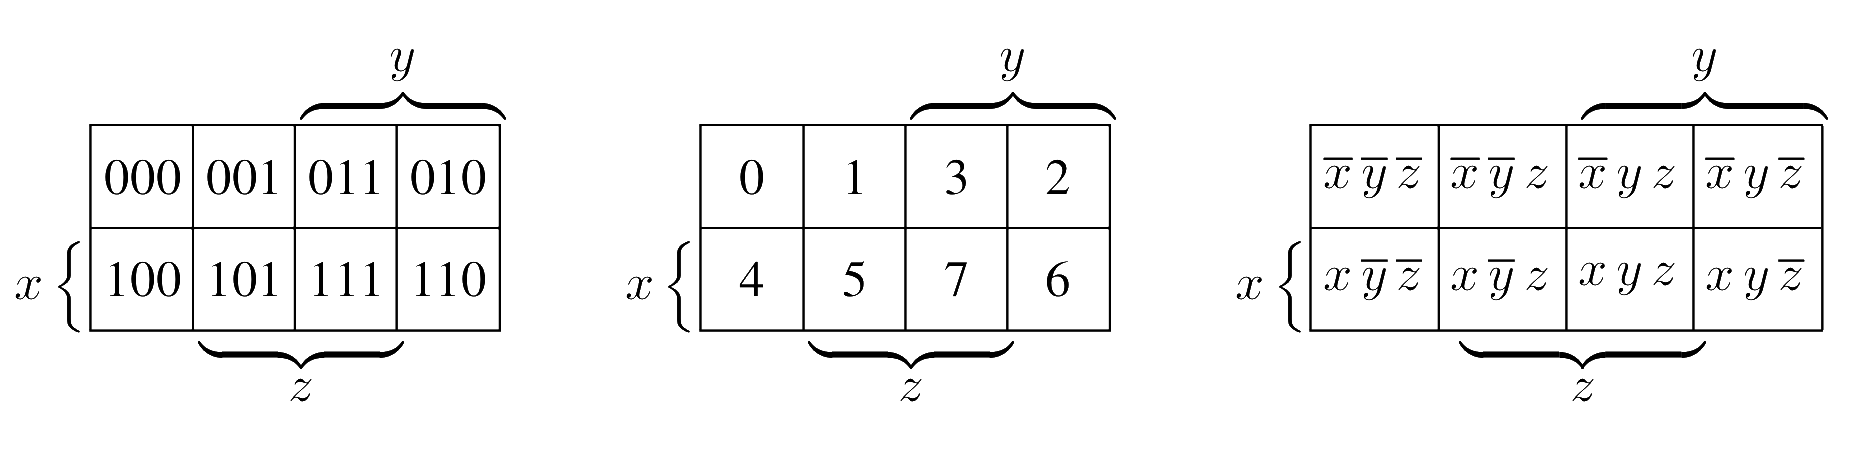
\includegraphics[width=\linewidth]{karnaugh/3-vars.png}
    \end{center}

    \noindent W polach odpowiadających liczbom z naszej funkcji wpisujemy \texttt{1}: \\

    \begin{center}
        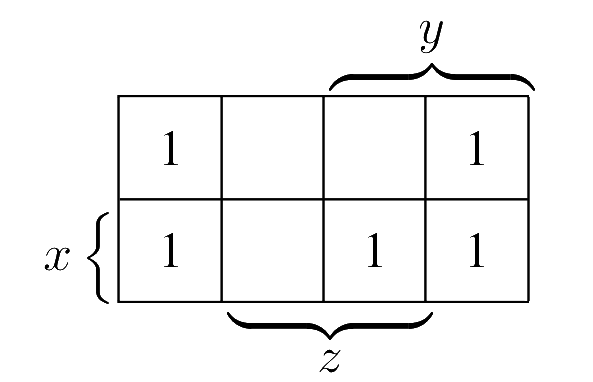
\includegraphics[width=0.7\linewidth]{karnaugh/1.png}
    \end{center}

    \noindent Nastepnie zaznaczamy prostokątnym zaznaczeniem jak największą liczbę pól z \texttt{1}, ale tylko w taki sposób aby liczba tych pól była całkowitą potęgą 2.
    Warto w tym miejscu pamiętać, że tablice Karnaugha możemy traktować jako tablicę cykliczną: \\

    \begin{center}
        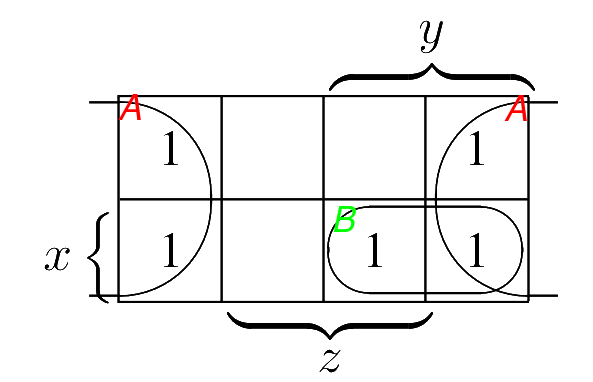
\includegraphics[width=0.7\linewidth]{karnaugh/2.png}
    \end{center}

    \noindent Następnie odczytujemy z tablic uproszczone już iloczyny dla poszczególnych zaznaczeń: dane zaznaczenie jest iloczynem tych zmiennych do których to zaznaczenie całkowicie należy lub nie należy. \\
    \noindent Tak więc dla zaznaczenia \textbf{\color[HTML]{ff0000}A} będzie to $\bar{z}$ ponieważ zaznaczenie w całości nie leży w obszarze zmiennej z. \\
    \noindent Natomiast dla zaznaczenia \textbf{\color[HTML]{00ff00}B} będzie to \texttt{xy} ponieważ leży ono całkowicie na obszarze zmiennych x oraz y. \\

    \noindent Ostatecznie nasza wyjściowa funkcja po uproszczeniu będzie miała postać sumy iloczynów poszczególnych obszarów: \\
    \noindent f(x, y, z) = $\sum$(0, 2, 4, 6, 7) = xy + $\bar{z}$

    \newpage

    \section{Programowalne układy logiczne PLD (ROM, PAL, PLA).}
    \section{Schemat blokowy komputera (maszyna von Neumanna).}
    \section{Zarządzanie procesami: stany procesu, algorytmy szeregowania z wywłaszczaniem.}
    \section{Muteks, semafor, monitor jako narzędzia synchronizacji procesów.}
    \section{Pamięć wirtualna i mechanizm stronicowania.}
    \section{Systemy plikowe - organizacja fizyczna i logiczna (na przykładzie wybranego systemu uniksopodobnego).}
    \section{Model ISO OSI. Przykłady protokołów w poszczególnych warstwach.}

    \newpage

    \section{Adresowanie w protokołach IPv4 i IPv6.}

    \subsection{Adresowanie w IPv4.}

    \begin{exercise}
        Wylicz adres sieci i broadcast z adresu hosta:
        \begin{enumerate}
            \item 11.12.13.14/24
            \item 11.12.13.14/25
            \item 11.12.13.167/28
            \item 11.12.138.167/17
        \end{enumerate}
    \end{exercise}

    \begin{enumerate}
        \item 11.12.13.14/24\\
        Maska $24 = 3*8$ bitów (24 jedynki i 8 zer) od lewej - odcina trzy pierwsze oktety. Dla adresu sieci zerujemy
        resztę, dla broadcastu - wypełniamy jedynkami.
        \begin{itemize}
            \item sieć: 11.12.13.0/24
            \item broadcast: 11.12.13.255/24
        \end{itemize}
        \item 11.12.13.14/25\\
        Maska 25 bajtów ``odcina'' pierwszy bit ostatniego oktetu (\textbf{0}0001110).
        Uzupełniamy zerami/jedynkami pozostałe 7 bitów.
        \begin{itemize}
            \item sieć: 11.12.13.0/24
            \item broadcast: 11.12.13.127/24
        \end{itemize}
        \item 11.12.13.167/28\\
        28 bitów - odcięte pierwsze z lewej cztery bity ostatniego oktetu (\textbf{1010}0111), pozostałe cztery uzupełniamy.
        \begin{itemize}
            \item sieć: 11.12.13.160/24
            \item broadcast: 11.12.13.175/24
        \end{itemize}
        \item 11.12.138.167/17\\
        17 bitów z lewej - zahaczamy jednym bitem o 3 oktet(\textbf{1}0001010), zostaje 15 bity.
        \begin{itemize}
            \item sieć: 11.12.128.0/24
            \item broadcast: 11.12.255.255/24
        \end{itemize}
    \end{enumerate}

    \begin{exercise}
        Podziel podaną sieć na jak najwięcej podsieci tak, aby każda miała n użytecznych adresów.
        \begin{enumerate}
            \item 10.0.0.0/24, n = 7
            \item 132.168.0.0/16, n = 30
        \end{enumerate}
    \end{exercise}

    \begin{enumerate}
        \item 10.0.0.0/24, n = 7\\
        7 użytecznych adresów IP - $7 \leq 2^k - 2 ~ \Rightarrow ~ 9 \leq 2^k ~ \Rightarrow ~ k = 4$. Potrzebujemy czterech
        bitów na adres hosta, zostają 4 bity na adres podsieci (pierwsze 24 odcina maska jako adres sieci). Nowa maska
        $= 24 + 4 = 28$ bajtów. Zatem adresy podsieci:
        \begin{itemize}
            \item pierwsza: 10.0.0.0/28
            \item druga: 10.0.0.16/28
            \item $\vdots$
            \item przedostatnia: 10.0.0.224/28
            \item ostatnia: 10.0.0.240/28
        \end{itemize}

        \item 132.168.0.0/16, n = 30\\
        $30 \leq 2^k - 2 ~ \Rightarrow ~ 32 \leq 2^k ~ \Rightarrow ~ k = 5$. 5 bitów na adres hosta, $32-5-16 = 11$ na adres
        podsieci - zaczynając od trzeciego oktetu. Nowa maska $= 16 + 11 = 27$.
        \begin{itemize}
            \item pierwsza: 132.168.0.0/27
            \item druga: 132.168.0.32/27
            \item $\vdots$
            \item przedostatnia: 132.168.255.224/27
            \item ostatnia: 132.168.255.192/27
        \end{itemize}
    \end{enumerate}

    \begin{exercise}
        Podziel daną sieć na n podsieci po równo hostów.
        \begin{enumerate}
            \item 132.168.0.0/16, n = 7
            \item 192.168.128.0/20, n = 4
        \end{enumerate}
    \end{exercise}

    \begin{enumerate}
        \item 132.168.0.0/16, n = 7\\
        $7 \leq 2^n ~ \Rightarrow ~ k = 3$ potrzebujemy 3 bitów na zakodowanie podsieci (będzie ich 8). 16 bitów odcina
        maska, kolejne 3 to podsieć i pozostałe 13 to host (nowa maska $= 16 + 3 = 19$).
        \begin{itemize}
            \item pierwsza: 132.168.0.0/19
            \item druga: 132.168.32.0/19
            \item $\vdots$
            \item przedostatnia: 132.168.192.0/19
            \item ostatnia: 132.168.224.0/19
        \end{itemize}

        \item 192.168.128.0/20, n = 4\\
        $4 \leq 2^k ~ \Rightarrow ~ k = 2$ bity na podsieć. 20 bitów odciętych przez maskę (w tym pierwsze cztery
        z 3 oktetu - \textbf{1000}0000), 2 na podsieć (nowa maska $=20+2=22$), 10 na adres hosta. Kolejne adresy:
        \begin{itemize}
            \item 192.168.128.0/22
            \item 192.168.132.0/22
            \item 192.168.136.0/22
            \item 192.168.140.0/22
        \end{itemize}
    \end{enumerate}

    \begin{exercise}
        \textbf{Sumaryzacja sieci}. Zagreguj poniższe sieci - wyznacz najbardziej precyzyjną agregującą ``nadsieć''.
        \begin{enumerate}
            \item
            \begin{enumerate}[label=(\Alph*)]
                \item 11.12.1.0/24
                \item 11.12.2.0/24
                \item 11.12.3.0/24
                \item 11.12.4.0/24
            \end{enumerate}
            \item
            \begin{enumerate}[label=(\Alph*)]
                \item 192.130.0.0/16
                \item 192.137.0.0/16
                \item 192.138.0.0/16
            \end{enumerate}
        \end{enumerate}
    \end{exercise}

    \begin{enumerate}
        \item
        \begin{enumerate}[label=(\Alph*)]
            \item 11.12.1.0/24
            \item 11.12.2.0/24
            \item 11.12.3.0/24
            \item 11.12.4.0/24
        \end{enumerate}
        Szukamy pierwsze od lewej bitu, który się różni dla co najmniej dwóch z tych sieci. Widzimy, że pierwsze dwa
        oktety są wspólne dla wszystkich, rozpisujemy więc trzeci:
        \begin{center}
            \begin{tabular}{c || c c c c c | c c c}
                A & \textbf{0} & \textbf{0} & \textbf{0} & \textbf{0} & \textbf{0} & 0 & 0 & 1\\
                \hline
                B & \textbf{0} & \textbf{0} & \textbf{0} & \textbf{0} & \textbf{0} & 0 & 1 & 0\\
                \hline
                C & \textbf{0} & \textbf{0} & \textbf{0} & \textbf{0} & \textbf{0} & 0 & 1 & 1\\
                \hline
                D & \textbf{0} & \textbf{0} & \textbf{0} & \textbf{0} & \textbf{0} & 1 & 0 & 0\\
                \hline
                \hline
                & 128 & 64 & 32 & 16 & 8 & 4 & 2 & 1\\
            \end{tabular}
        \end{center}
        Różnią się dopiero na 6 bicie, pierwsze pięć jest zgodnych. Zatem nadsieć współdzieli pierwsze $16+5=21$ bitów:
        \[11.12.0.0/21\]

        \item
        \begin{enumerate}[label=(\Alph*)]
            \item 192.130.0.0/16
            \item 192.137.0.0/16
            \item 192.138.0.0/16
        \end{enumerate}
    \end{enumerate}
    Różnica w drugim oktecie:
    \begin{center}
        \begin{tabular}{c || c c c c | c c c c}
            A & \textbf{1} & \textbf{0} & \textbf{0} & \textbf{0} & 0 & 0 & 1 & 0\\
            \hline
            B & \textbf{1} & \textbf{0} & \textbf{0} & \textbf{0} & 1 & 0 & 0 & 1\\
            \hline
            C & \textbf{1} & \textbf{0} & \textbf{0} & \textbf{0} & 1 & 0 & 1 & 0\\
            \hline
            \hline
            & 128 & 64 & 32 & 16 & 8 & 4 & 2 & 1\\
        \end{tabular}
    \end{center}
    Różnią się dopiero na 5 bicie, pierwsze cztery są zgodne. Zatem nadsieć współdzieli pierwsze $16+4=20$ bitów:
    \[192.128.0.0/21\]

    \newpage

    \section{Najważniejsze procesy zachodzące w sieci komputerowej od momentu wpisania adresu strony WWW do wyświetlenia strony w przeglądarce (komunikat HTTP, segment TCP, system DNS, pakiet IP, ARP, ramka).}
    \section{Działanie przełączników Ethernet, sieci VLAN, protokół STP.}
    \section{Rola routerów i podstawowe protokoły routingu (RIP, OSPF).}
    \section{Szyfrowanie z kluczem publicznym, podpis cyfrowy, certyfikaty.}
    \section{Wirtualne sieci prywatne, protokół IPsec.}


\end{document}